%%%%%%%%%%%%%%%%%%%%%%%%%%%%%%%%%%%%
%                                  %
% Titre  : m.tex                   %
% Sujet  : Maintenance manual      %
%          Document body           %
% Auteur : Francois Pellegrini     %
%                                  %
%%%%%%%%%%%%%%%%%%%%%%%%%%%%%%%%%%%%

%% Formatage et pagination.

\documentclass{article}
\usepackage{a4}
\usepackage[dvips]{graphicx}
%\documentstyle[11pt,a4,fullpage,epsf]{article}
%\textwidth      16.0cm
%\oddsidemargin   -0.5cm
%\evensidemargin  -0.5cm
%\marginparwidth  0.0cm
%\marginparsep    0.0cm
%\marginparpush   0.0cm
%\topmargin        0.5cm
%\headheight      0.0cm
%\headsep         0.0cm
%\textheight     25.0cm
%\footheight      0.0cm
%\footskip        0.0cm

\sloppy                                          % Gestion des overfull hbox
\renewcommand{\baselinestretch}{1.05}            % Hauteur lignes x 1.05

\setcounter{secnumdepth}{3}                      % Sous-sous-sections numerotees
\setcounter{tocdepth}{3}                         % Sous-sous-sections dans la table

%% Macros et commandes utiles.

\makeatletter
\@definecounter{enumv}                           % 8 niveaux d'itemizations
\@definecounter{enumvi}
\@definecounter{enumvii}
\@definecounter{enumviii}
\def\itemize{\ifnum \@itemdepth >8 \@toodeep\else \advance\@itemdepth \@ne
\edef\@itemitem{labelitem\romannumeral\the\@itemdepth}%
\list{\csname\@itemitem\endcsname}{\def\makelabel##1{\hss\llap{##1}}}\fi}
\let\enditemize =\endlist

\def\@iteme[#1]{\if@noparitem \@donoparitem      % Item long pour options
  \else \if@inlabel \indent \par \fi
         \ifhmode \unskip\unskip \par \fi
         \if@newlist \if@nobreak \@nbitem \else
                        \addpenalty\@beginparpenalty
                        \addvspace\@topsep \addvspace{-\parskip}\fi
           \else \addpenalty\@itempenalty \addvspace\itemsep
          \fi
    \global\@inlabeltrue
\fi
\everypar{\global\@minipagefalse\global\@newlistfalse
          \if@inlabel\global\@inlabelfalse
             \setbox\@tempboxa\hbox{#1}\relax
             \hskip \itemindent \hskip -\parindent
             \hskip -\labelwidth \hskip -\labelsep
             \ifdim \wd\@tempboxa > \labelwidth
               \box\@tempboxa\hfil\break
             \else
               \hbox to\labelwidth{\box\@tempboxa\hfil}\relax
               \hskip \labelsep
             \fi
             \penalty\z@ \fi
          \everypar{}}\global\@nobreakfalse
\if@noitemarg \@noitemargfalse \if@nmbrlist \refstepcounter{\@listctr}\fi \fi
\ignorespaces}
\def\iteme{\@ifnextchar [{\@iteme}{\@noitemargtrue \@iteme[\@itemlabel]}}

\let\@Hxfloat\@xfloat
\def\@xfloat#1[{\@ifnextchar{H}{\@HHfloat{#1}[}{\@Hxfloat{#1}[}}
\def\@HHfloat#1[H]{%
\expandafter\let\csname end#1\endcsname\end@Hfloat
\vskip\intextsep\def\@captype{#1}\parindent\z@
\ignorespaces}
\def\end@Hfloat{\vskip \intextsep}
\makeatother

\newcommand{\bn}{\begin{displaymath}}            % Equations non-numerotees
\newcommand{\en}{\end{displaymath}}
\newcommand{\bq}{\begin{equation}}               % Equations numerotees
\newcommand{\eq}{\end{equation}}

\newcommand{\lbo}{\linebreak[0]}
\newcommand{\lbt}{\linebreak[2]}
\newcommand{\noi}{{\noindent}}                   % Pas d'indentation
\newcommand{\spa}{{\protect \vspace{\bigskipamount}}} % Espace vertical

\newcommand{\eg}{{\it e\@.g\@.\/\ }}             % e.g.
\newcommand{\ie}{{\it i\@.e\@.\/\ }}             % i.e.

\newcommand{\scotch}{{\sc Scotch}}               % "scotch"
\newcommand{\libscotch}{{\sc libScotch}}         % "libscotch"
\newcommand{\ptscotch}{\textsc{PT-Scotch}}       % "PT-Scotch"
\newcommand{\libptscotch}{{\sc libPTScotch}}     % "libPTScotch"

\newcommand{\UB}{{\rm UB}}                       % UB

%% Version du document.

\newcommand{\scotchver}{6.1}
\newcommand{\scotchversub}{6.1.3}

%% Page de garde.

\begin{document}

\date{\today}

\title{
\includegraphics{../misc/scotch_logo_color.ps}\\[1em]
       {\LARGE\bf \libscotch\ \textsc{\scotchver} Maintainer's Guide}\\[1em]}

\author{Fran\c cois Pellegrini\\
Universit\'e de Bordeaux \& LaBRI, UMR CNRS 5800\\
TadAAM team, INRIA Bordeaux Sud-Ouest\\
351 cours de la Lib\'eration, 33405 TALENCE, FRANCE\\
{\tt francois.pellegrini@u-bordeaux.fr}}

\maketitle

\begin{abstract}
This document describes some internals of the \libscotch\
library.
\end{abstract}

\clearpage

\tableofcontents

%%%%%%%%%%%%%%%%%%%%%%%%%%%%%%%%%%%%
%                                  %
% Titre  : s_i.tex                 %
% Sujet  : Manuel de maintenance   %
%          du projet 'Scotch'      %
%          Introduction            %
% Auteur : Francois Pellegrini     %
%                                  %
%%%%%%%%%%%%%%%%%%%%%%%%%%%%%%%%%%%%

\section{Introduction}

This document is a starting point for the persons interested in using
\scotch\ as a testbed for their new partitioning methods, and/or
willing to contribute to it by making these methods available to the
rest of the scientific community.

Much information is missing. If you need specific information, please
send an e-mail, so that relevant additional information can be added
to this document.
                                  % Introduction
%%%%%%%%%%%%%%%%%%%%%%%%%%%%%%%%%%%%
%                                  %
% Titre  : m_n.tex                 %
% Sujet  : Maintenance manual of   %
%          Scotch                  %
%          Style and naming        %
%          conventions             %
% Auteur : Francois Pellegrini     %
%                                  %
%%%%%%%%%%%%%%%%%%%%%%%%%%%%%%%%%%%%

\section{Coding style}

The \scotch\ coding style is now well established. Hence, potential
contributors are requested to abide by it, to provide a global ease of
reading while browsing the code, and to ease the work of their
followers.

In this section, the numbering of the characters of each line is
assumed to start from zero.

\subsection{Typing}

\subsubsection{Spacing}

Expressions are like sentences, where words are separated by
spaces. Hence, an expression like ``\texttt{if~(n == NULL)~\{}''
reads: ``if $n$ is-equal-to NULL then'', with words separated by
single spaces.

As in standard typesetting, there is no space after an opening
parenthesis, nor before a closing one, because they are not words.

When it follows a keyword, an opening brace is always on the same line
as the keyword (save for special cases, e.g. preprocessing macros
between the keyword and the opening brace). This is meant to maximize
the number of ``useful readable lines'' on the screen. However,
closing braces are on a separate line, aligned with the indent of the
line that contains the matching opening brace. This is meant to find
in a glance the line that contains this opening brace.

Brackets are not considered as words: they are stuck both to the word
on their left and the word on their right.

Reference and dereference operators ``\texttt{\&}'' and ``\texttt{*}''
are stuck to the word on their right. However, the multiplication
operator ``\texttt{*}'' counts as a word in arithmetic expressions.

Semicolons are always stuck to the word on their left, except when
they follow an empty instruction, e.g., an empty loop body or an empty
\texttt{for} field. Empty instructions are materialized by a single
space character, which makes the semicolon separated from the
preceding word. For instance: ``\texttt{for~(~;~;~)~;}''.

Ternary operator elements ``\texttt{?}'' and ``\texttt{:}'' are
considered as words and are surrounded by spaces. When the ternary
construct spans across multiple lines, they are placed at the
beginning of each line, before the expression they condition, and not
at the end of the previous line.

\subsubsection{Aligning}

When several consecutive lines contain similar expressions that are
strongly connected, e.g. arguments of a \texttt{mem\lbt Alloc\lbt
  Group()} routine, or assignments of multiple fields of the same
structure(s), extra spaces can be added to align parts of the
expressions. This is a matter of style and opportunity.

For instance, when consecutive lines contain function calls where
opening parentheses are close to each other and their arguments
overlap, open parentheses have to be aligned. However, when arguments
do not overlap, alignment is not required (e.g., for \texttt{return}
statements with small parameters).

\subsubsection{Idiomatic specificities}

While, in C, \texttt{return} is a keyword which does not need
parentheses around its argument, the \scotch\ coding style treats it
as if it were a function call, thus requiring parentheses around its
argument when it has one.

\subsection{Indenting}

Indenting is subject to the following rules:
\begin{itemize}
\item
  All indents are of two characters. Hence, starting from column zero,
  all lines start at even column numbers.
\item
  Tabs are never used in the source code. If your text editor replaces
  chunks of spaces by tabs, it is your duty to disable this feature or
  to make sure to replace all tabs by spaces before the files are
  committed. Unwanted tabs are shown in red when performing a
  ``\texttt{git diff}'' prior to committing.
\end{itemize}

Condition bodies are always indented on the line below the condition
statement. ``\texttt{if}'' statements are always placed at the beginning
of a new line, except when used as an ``\texttt{else~if}''
construct, in which the two keywords appear on the same line,
separated by a single space.

Loop bodies are always indented on the line below the loop statement,
except when the loop body is an empty instruction. In this case, the
terminating semicolon is placed on the same line as the loop
statement, after a single space.

\subsection{Comments}

All comments are C-style, that is, of the form
``\texttt{/*}$\ldots$\texttt{*/}''. C++-style comments should never be
used.

There are three categories of comments: file comments, function/data
structure comments, and line comments. Commenting is subject to the
following rules:
\begin{itemize}
\item
  File comments are standard header blocks that must be copied as
  is. Hence, there is little to say about them. On top of each file
  should be placed a license header, which depends on the origin of
  the file.
\item
  Block comments start with ``\texttt{/*}'' and end with
  ``\texttt{*/}'' on a separate subsequent line. Intermediate lines
  start with ``\texttt{**}''. All these comment markers are placed at
  colums zero. Comment text is separated from the comment markers by a
  single space character. Text in block comments is made of titles or
  of full sentences, that are terminated with a punctuation sign (most
  often a final dot).
\item
  Line comments are of two types: structure definition line comments
  in header files, and code line comments.

  Structure definition line comments in header files start with
  ``\texttt{/*+}'' and end with ``\texttt{+*/}''. This is an old
  Doxygen syntax, which has been preserved over time. Code line
  comments start classically with ``\texttt{/*}'' and end with
  ``\texttt{*/}''.

  All these comments start at least at character~$50$. If the C code
  line is longer, comment lines start one character after the end of
  the line, after a single space. End comment markers are placed at
  least one character after the end of the comment text. When several
  line comments are present on consecutive lines, comment terminators
  are aligned to the farthest comment terminator.

  Comment text always starts with an uppercase letter, and have no
  terminating punctuation sign. They are written in the imperative
  mode, and a positive form (no question asked).

  Line comments for C pre-processing conditional macros
  (e.g. ``\texttt{\#else}'' or ``\texttt{\#endif}'') are not subject
  to indentation rules. They start one character after the keyword,
  and are not subject to end marker alignment, except when consecutive
  lines bear the same keyword (\textit{i.e.}, a ``\texttt{\#endif}''
  statement).
\end{itemize}

\section{Naming conventions}
\label{sec-naming}

Data types, variables, structure fields and function names follow
strict naming conventions. These conventions strongly facilitate the
understanding of the meaning of the expressions, and prevent from
coding mistakes. For instance, ``\texttt{verttax[edgenum]}'' would
clearly be an invalid expression, as a vertex array cannot be indexed
by an edge number. Hence, potential contributors are required to
follow them strictly.

\subsection{File inclusion markers}
\label{sec-naming-file-inclusion-markers}

File inclusion markers are \texttt{\#define}'s which indicate that a
given source file (either a ``\texttt{.c}'' source code file or a
``\texttt{.h}'' header file) has been already encountered.

To minimize risks of collisions with symbols of external libraries,
file inclusion markers start with a prefix that represents the name of
the project, followed by the name of the file in question (without its
type suffix). While filenames can be long, this is not an issue since
the length of the significant part of C~preprocessor symbols is at
least 63~characters\footnote{See e.g.
\url{https://gcc.gnu.org/onlinedocs/cpp/Implementation-limits.html}},
thus longer than that of C identifiers, which is 32~characters.
Header file marker identifiers are suffixed with ``\texttt{\_H}'',
while C source file markers have no suffix.

In order to further minimize risks of collisions, file inclusion
markers should be placed in a file only when needed, that is, when
effectively used as the parameter of a conditional inclusion statement
within another source file.

The current project prefixes are:
\begin{itemize}
\item
  \texttt{SCOTCH\_}: the \scotch\ project itself;
\item
  \texttt{ESMUMPS\_}: the \esmumps\ library, which is treated as a
  separate project to avoid conflicts with data structures and files
  that exist in both libraries, such as \texttt{Graph}'s.
\end{itemize}

\subsection{Variables and fields}
\label{sec-naming-variables}

Variables and fields of the sequential \scotch\ software are commonly
built from a radical and a suffix. When contextualization is required,
e.g., the same kind of variable appear in two different objects, a
prefix is added. In \ptscotch, a second radical is commonly used, to
inform on variable locality or duplication across processes.

Common radicals are:
\begin{itemize}
\item
\texttt{vert}: vertex.
\item
\texttt{velo}: vertex load.
\item
\texttt{vnum}: vertex number, used as an index to access another vertex
structure. This radical typically relates to an array that contains
the vertex indices, in some original graph, corresponding to the
vertices of a derived graph (e.g., an induced graph).
\item
\texttt{vlbl}: user-defined vertex label (at the user API level).
\item
\texttt{edge}: edge (\texttt{i.e.}, arcs, in fact).
\item
\texttt{edlo}: edge (arc) load.
\item
\texttt{arch}: target architecture.
\item
\texttt{graf}: graph.
\item
\texttt{mesh}: mesh.
\end{itemize}

Common suffices are:
\begin{itemize}
\item
\texttt{bas}: start ``based'' value for a number range; see the
``\texttt{nnd}'' suffix below. For number basing and array indexing,
see Section~\ref{sec-basing}.
\item
\texttt{end}: vertex end index of an edge (e.g.,
\texttt{vertend}, wrt. \texttt{vertnum}). The \texttt{end} suffix is
a sub-category of the \texttt{num} suffix.
\item
\texttt{nbr}: number of instances of objects of a given radical
type (e.g., \texttt{vertnbr}, \texttt{edgenbr}). They are commonly
used within ``un-based'' loop constructs, such as:
``\texttt{for (vertnum = 0; vertnum < vertnbr; vertnum ++)} \ldots''.
\item
\texttt{nnd}: end based value for a number range, commonly used
for loop boundaries. Usually, $\mbox{*\texttt{nnd}} =
\mbox{*\texttt{nbr}} + \mbox{\texttt{baseval}}$. For instance,
$\mbox{\texttt{vertnnd}} = \mbox{\texttt{vertnbr}} +
\mbox{\texttt{baseval}}$. They are commonly used in based loop
constructs, such as:
``\texttt{for (vertnum = baseval; vertnum < vertnnd; vertnum ++)}
\ldots''. For local vertex ranges, e.g., within a thread that manages
only a partial vertex range, the loop construct would be:
``\texttt{for (vertnum = vertbas; vertnum < vertnnd; vertnum ++)}
\ldots''.
\item
\texttt{num}: based or un-based number (index) of some instance of an
object of a given radical type. For instance, \texttt{vertnum} is the
index of some (graph) vertex, that can be used to access adjacency
(\texttt{verttab}) or vertex load (\texttt{velotab}) arrays.
$0 \leq \mbox{\texttt{vertnum}} < \mbox{\texttt{vertnbr}}$ if the
vertex index is un-based, and $\mbox{\texttt{baseval}} \leq
\mbox{\texttt{vertnum}} < \mbox{\texttt{vertnnd}}$
if the index is based, that it, counted starting from
\texttt{baseval}.
\item
\texttt{ptr}: pointer to an instance of an item of some radical type
(e.g., \texttt{grafptr}).
\item
\texttt{sum}: sum of several values of the same radical type (e.g.,
\texttt{velosum}, \texttt{edlosum}).
\item
\texttt{tab}: reference to the first memory element of an array. Such
a reference is returned by a memory allocation routine (e.g.,
\texttt{mem\lbt Alloc}) or allocated from the stack.
\item
\texttt{tax} (for ``\textit{table access}''): reference to an array
that will be accessed using based indices. See
Section~\ref{sec-basing}.
\item
\texttt{tnd}: pointer to the based after-end of an array of items
of radix type (e.g. \texttt{velotnd}). Variables of this suffix are
mostly used as bounds in loops.
\item
\texttt{val}: value of an item. For instance, \texttt{baseval} is the
indexing base value, and \texttt{veloval} is the load of some vertex,
that may have been read from a file.
\end{itemize}

Common prefixes are:
\begin{itemize}
\item
\texttt{src}: source, wrt. active. For instance, a source graph is a
plain \texttt{Graph} structure that contains only graph topology,
compared to enriched graph data structures that are used for specific
computations such as bipartitioning.
\item
\texttt{act}: active, wrt. source. An active graph is a data structure
enriched with information required for specific computations, e.g. a
\texttt{Bgraph}, a \texttt{Kgraph} or a \texttt{Vgraph} compared to a
\texttt{Graph}.
\item
\texttt{ind}: induced, wrt. original.
\item
\texttt{src}: source, wrt. active or target.
\item
\texttt{org}: original, wrt. induced. An original graph is a graph
from which a derived graph will be computed, e.g. an induced subgraph.
\item
\texttt{tgt}: target.
\item
\texttt{coar}: coarse, wrt. fine (e.g. \texttt{coarvertnum}, as a
variable that holds the number of a coarse vertex, within some
coarsening algorithm).
\item
\texttt{fine}: fine, wrt. coarse.
\item
\texttt{mult}: multinode, for coarsening.
\end{itemize}

\subsection{Functions}
\label{sec-naming-functions}

Like variables, routines of the \scotch\ software package follow a
strict naming scheme, in an object-oriented fashion. Routines are
always prefixed by the name of the data structure on which they
operate, then by the name of the method that is applied to the said
data structure. Some method names are standard for each class.

Standard method names are:
\begin{itemize}
\item
\texttt{Alloc}: dynamically allocate an object of the given class. Not
always available, as many objects are allocated on the stack as local
variables.
\item
\texttt{Init}: initialization of the object passed as parameter.
\item
\texttt{Free}: freeing of the external structures of the object, to save
space. The object may still be used, but it is considered as ``empty''
(e.g., an empty graph). The object may be re-used after it is
initialized again.
\item
\texttt{Exit}: freeing of the internal structures of the object. The
object must not be passed to other routines after the \texttt{Exit}
method has been called.
\item
\texttt{Copy}: make a fully operational, independent, copy of the
object, like a ``clone'' function in object-oriented languages.
\item
\texttt{Load}: load object data from stream.
\item
\texttt{Save}: save object data to stream.
\item
\texttt{View}: display internal structures and statistics, for debugging
purposes.
\item
\texttt{Check}: check internal consistency of the object data, for
debugging purposes. A \texttt{Check} method must be created for any
new class, and any function that creates or updates an instance of
some class must call the appropriate \texttt{Check} method, when
compiled in debug mode.
\end{itemize}

\subsection{Array index basing}
\label{sec-basing}

The \libscotch\ library can accept data structures that come both from
FORTRAN, where array indices start at $1$, and C, where they start at
$0$. The start index for arrays is called the ``base value'', commonly
stored in a variable (or field) called \texttt{baseval}.

In order to manage based indices elegantly, most references to arrays
are based as well. The ``table access'' reference, suffixed as
``\texttt{tax}'' (see Section~\ref{sec-naming-variables}), is defined
as the reference to the beginning of an array in memory, minus the
base value (with respect to pointer arithmetic, that is, in terms of
bytes, times the size of the array cell data type). Consequently, for
any array whose beginning is pointed to by \texttt{xxxxtab}, we have
$\mbox{\texttt{xxxxtax}} = \mbox{\texttt{xxxxtab}} - \mbox{\texttt{baseval}}$.
Consequently \texttt{xxxxtax[baseval]} always represents the first
cell in the array, whatever the base value is.
Of course, memory allocation and freeing operations must always
operate on \texttt{tab} pointers only.

In terms of indices, if the size of the array is \texttt{xxxxnbr},
then
$\mbox{\texttt{xxxxnnd}} = \mbox{\texttt{xxxxnbr}} + \mbox{\texttt{baseval}}$,
so that valid indices \texttt{xxxxnum} always belong to the range
$[\mbox{\texttt{baseval}};\mbox{\texttt{vertnnd}}[$. Consequently,
loops often take the form:
\begin{center}
{\renewcommand{\baselinestretch}{1.05}
\footnotesize\tt
\begin{verbatim}
  for (xxxxnum = baseval; xxxxnum < xxxxnnd; xxxxnum ++) {
    xxxxtax[xxxxnum] = ...;
  }
\end{verbatim}
}
\end{center}
                                  % Naming conventions
%%%%%%%%%%%%%%%%%%%%%%%%%%%%%%%%%%%%
%                                  %
% Titre  : m_s.tex                 %
% Sujet  : Manuel de maintenance   %
%          du projet 'Scotch'      %
%          Structure generale      %
% Auteur : Francois Pellegrini     %
%                                  %
%%%%%%%%%%%%%%%%%%%%%%%%%%%%%%%%%%%%

\section{General structure of the \libscotch\ library}
\label{sec-structure}

\subsection{Naming conventions}

All of the files of the \scotch\ project have been written using
strict coding conventions, to ease maintenance and further extension
by external contributors. Therefore, contributors are {\bf strongly}
invited to follow these coding conventions so as to ease the work of
their followers.

\subsubsection{Variables}

Variables are named by specialization, with prefixes and suffixes.

Common prefixes are:
\begin{itemize}
\item
act : active, wrt. source
\item
src : source, wrt. active
\item
tgt : target.
\item
coar : coarse, wrt. fine.
\item
fine : fine, wrt. coarse.
\item
mult : multinode, for coarsening.
\end{itemize}

Common radicals are:
\begin{itemize}
\item
vert : vertex.
\item
velo : vertex load.
\item
vnum : vertex number, used as index, for instance in {\tt vnumtab}).
\item
vlbl : vertex label (for interface).
\item
edge : edge.
\item
edlo : edge load.
\end{itemize}

Common suffices are:
\begin{itemize}
\item
{\tt nbr} : number of (instances of).
\item
{\tt num} : number of some instance of.
\item
{\tt val} : value of.
\item
{\tt sum} : sum of several values of.
\item
{\tt tab} : pointer to the first memory element of an array of, for
instance as returned by a {\tt mem\lbt Alloc} routine.
\item
{\tt tax} : (for ``{\it table access}'') pointer to the first element
of an array that is to be accessed by means of based indices. The
\libscotch\ library can accept data structures that come both from
FORTRAN, where array indices start at $1$, and C, where they start at
$0$. By accessing ``{\tt tax}'' arrays, where the {\tt tax} pointer is
equal to the {\tt tab} pointer minus the value of the indexing base,
this is completely transparent for coding, save for memory allocation
and freeing operations, which must operate on {\tt tab} pointers only.
\item
{\tt tnd} : pointer to the end of an array of (mostly used as a bound
in loops).
\item
{\tt ptr} : pointer to an instance of.
\end{itemize}

For instance, {\tt coarvertnum} is a variable that holds the number of
a coarse vertex, within some coarsening algorithm. It is also easy to
guess how to name a variable that holds a pointer to an active edge.

\subsubsection{Functions}

Routines that operate on data structures are named by specialization,
from the name of the structure type they apply to.

Common suffixes are:
\begin{itemize}
\item
{\tt Init} : initialization of a structure (object) passed as parameter.
\item
{\tt Free} : freeing of the external structures of the object, to save
space. The object may still be used after it is initialized again.
\item
{\tt Exit} : freeing of the internal structures of the object. The
object must not be passed to other routines after the {Exit} method
has been called.
\item
{\tt Copy} : make a fully operational, independent, copy of the object.
\item
{\tt Load} : load from stream.
\item
{\tt Save} : save to stream.
\item
{\tt View} : display internal structures and statistics, for debugging
purposes.
\item
{\tt Check} : check internal coherence, for debug.
\end{itemize}

\subsection{Structure of the library}

%\subsubsection{Modules}

All of the routines that comprise the \libscotch\ libraries are
grouped by the type of data structure onto which they apply and by
function, in an object-oriented manner. This organization is reflected
into the naming and contents of all of the source files.

The main modules of the \libscotch\ library are the following :
\begin{itemize}
\item
{\tt arch} : target architectures used by the static mapping methods.
\item
{\tt bgraph} : graph edge bipartitioning methods.
\item
{\tt graph} : basic graph handling methods.
\item
{\tt hgraph} : graph ordering methods. These are based on an extended
``halo'' graph structure, thus for the name.
\item
{\tt hmesh} : mesh ordering methods.
\item
{\tt kgraph} : k-way graph partitioning methods.
\item
{\tt library} : interface routines for the \libscotch\ library.
\item
{\tt mapping} : definition of the mapping structure.
\item
{\tt mesh} : basic mesh handling methods.
\item
{\tt order} : definition of the ordering structure.
\item
{\tt parser} : strategy parsing routines, based on a Lex-Yacc
parser.
\item
{\tt vgraph} : graph vertex bipartitioning methods.
\item
{\tt vmesh} : mesh node bipartitioning methods.
\end{itemize}

Each of the file names is prefixed by the name of the module, followed
by one or two words that describe the type of action performed by the
routines of the file.
For instance, in module {\tt bgraph} :
\begin{itemize}
\item
{\tt bgraph.h} is the header file that defines the {\tt bgraph}
structure,
\item
{\tt bgraph\_bipart\_fm.[ch]} are the files that contain the
Fiduccia-Mattheyses-like graph bipartitioning method,
\item
{\tt bgraph\_check.c} is the file that contains the consistency
checking routine for {\tt Bgraph} structures,
\end{itemize}
and so on. Every source file has a comments header briefly describing
the purpose of the routines it contains.

%This section lists the main structures used within \libscotch. Each of
%these is defined in a C header file of same name in the {\tt
%libscotch\_\lbt 4.x/\lbo src} directory. For instance, the {\tt Graph}
%structure is defined in file {\tt graph.h}, the {Vmesh} structure is
%defined in file {\tt vmesh.h}, and so on.
                                  % Structure of the libScotch
%%%%%%%%%%%%%%%%%%%%%%%%%%%%%%%%%%%%
%                                  %
% Titre  : m_f.tex                 %
% Sujet  : Maintenance manual of   %
%          Scotch                  %
%          File formats v6.0       %
% Auteur : Francois Pellegrini     %
%                                  %
%%%%%%%%%%%%%%%%%%%%%%%%%%%%%%%%%%%%

\section{Files and data structures}
\label{sec-file}

User-manageable file formats are described in the \scotch user's
guide. This section contains information that are relevant only to
developers and maintainers.

For the sake of portability, readability, and reduction of storage space,
all the data files shared by the different programs of the
\scotch\ project are coded in plain ASCII text exclusively.
Although one may speak of ``lines'' when describing file formats,
text-formatting characters such as newlines or tabulations are not
mandatory, and are not taken into account when files are read.
They are only used to provide better readability and understanding.
Whenever numbers are used to label objects, and unless explicitely
stated, \textbf{numberings always start from zero}, not one.

\subsection{Decomposition-defined architecture files}
\label{sec-file-target-deco-one}

Decomposition-defined architecture files are the way to describe
irregular target architectures that cannot be represented as
algorithmically-coded architectures.

Two main file formats coexist: the ``\texttt{deco 0}'' and
``\texttt{deco 2}'' formats. ``\texttt{deco}'' stands for
``decomposition-defined architecture'', followed by the format
number. The ``\texttt{deco 1}'' format is a compiled form of the
``\texttt{deco 0}'' format. We will describe it here.

The ``\texttt{deco 1}'' file format results from an $O(p^2)$
preprocessing of the ``\texttt{deco 0}'' target architecture
format. While the ``\texttt{deco 0}'' format contains a distance
matrix between all pairs of terminal domains, which is consequently in
in $\Theta(p^2/2)$, the ``\texttt{deco 1}'' format contains the
distance matrix between any pair of domains, whether they are terminal
or not. Since there are roughly $2p$ non-terminal domains in a
target architecture with $p$ terminal domains, because all domains
form a binary tree whose leaves are the terminal domains, the distance
matrix of a ``\texttt{deco 1}'' format is in $\Theta(2p^2)$, that is,
four times that of the corresponding ``\texttt{deco 0}'' file.

Also, while the ``\texttt{deco 0}'' format lists only the
characteristics of terminal domains (in terms of weights and labels),
the ``\texttt{deco 1}'' format provides these for all domains, so as
to speed-up the retrieval of the size, weight and label of any domain,
whether it is terminal or not.

The ``\texttt{deco 1}'' header is followed by two integer numbers,
which are the number of processors and the largest terminal number used
in the decomposition, respectively (just as for ``\texttt{deco 0}''
files). Two arrays follow.

The first array has as many lines as there are domains (and not only
terminal domains as in the case of ``\texttt{deco 0}'' files). Each of
these lines holds three numbers: the label of the terminal domain that
is associated with this domain (which is the label of the terminal
domain of smallest number contained in this domain), the size of the
domain, and the weight of the domain.
The first domain in the array is the initial domain holding all the
processors, that is, domain $1$. The other domains in the array are
the resulting subdomains, in ascending domain number order, such that
the two subdomains of a given domain of number $i$ are numbered $2i$
and $2i+1$.

The second array is a lower triangular diagonal-less matrix that gives the
distance between all pairs of domains.

For instance, Figure~\ref{fig-file-targetdeco-zero} and
Figure~\ref{fig-file-targetdeco-one} show the contents of the
``\texttt{deco 0}'' and ``\texttt{deco 1}'' architecture decomposition
files for $\UB(2,3)$, the binary de~Bruijn graph of dimension~$3$, as
computed by the \texttt{amk\_grf} program.
\begin{figure}[hbt]
\begin{tabular}{p{0.69\linewidth}@{}p{0.29\linewidth}}
\begin{center}
\parbox[t]{0.9\linewidth}{\vspace{0pt}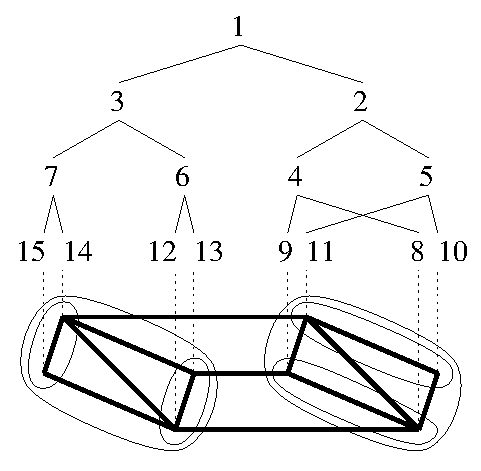
\includegraphics[width=0.7\linewidth]{s_f_d.ps}}
\end{center}
&
\begin{center}
{\renewcommand{\baselinestretch}{1.05}
\footnotesize\tt
\begin{verbatim}
deco 0
8	15
0	1	15
1	1	14
2	1	13
3	1	11
4	1	12
5	1	9
6	1	8
7	1	10
1
2 1
2 1 2
1 1 1 2
3 2 1 1 2
2 2 2 1 1 1
3 2 3 1 2 2 1
\end{verbatim}
}
\end{center}
\end{tabular}
\caption{``\texttt{deco 0}'' target decomposition file for $\UB(2,3)$.
         The terminal numbers associated with every processor define a unique
         recursive bipartitioning of the target graph.}
\label{fig-file-targetdeco-zero}
\end{figure}

\begin{figure}[hbt]
\begin{tabular}{p{0.49\linewidth}@{}p{0.49\linewidth}}
\begin{center}
{\renewcommand{\baselinestretch}{1.05}
\footnotesize\tt
\begin{verbatim}
deco
1
8	15
0	8	8
3	4	4
0	4	4
5	2	2
3	2	2
2	2	2
0	2	2
6	1	1
5	1	1
7	1	1
3	1	1
4	1	1
2	1	1
1	1	1
0	1	1
\end{verbatim}
}
\end{center}
&
\begin{center}
{\renewcommand{\baselinestretch}{1.05}
\footnotesize\tt
\begin{verbatim}
2	2	2	2	1	2	2	1
3	1	2	2	1	2	2	2
3	1	2	2	1	2	1	2
1	1	2	2	3	2	3	1
2	2	3	1	3	2	3	2
1	3	3	1	2	2	1	2
1	1	2	2	1	1	1	2
2	1	2	2	1	1	1	2
2	2	3	3	2	2	3	1
2	2	1	3	2	1	2	2
1	2	2	1	1	2	2	2
1	1	1	3	3	2	3	3
2	1	2	3	3	2	1	2
1
\end{verbatim}
}
\end{center}
\end{tabular}
\caption{``\texttt{deco 1}'' target decomposition file for $\UB(2,3)$,
  compiled with the \texttt{acpl} tool from the ``\texttt{deco 0}''
  file displayed in Figure~\ref{fig-file-targetdeco-zero}.}
\label{fig-file-targetdeco-one}
\end{figure}
                                  % File formats
%%%%%%%%%%%%%%%%%%%%%%%%%%%%%%%%%%%%
%                                  %
% Title   : m_m.tex                %
% Subject : Maintenance manual of  %
%           Scotch                 %
%           How to add a method    %
% Author  : Francois Pellegrini    %
%                                  %
%%%%%%%%%%%%%%%%%%%%%%%%%%%%%%%%%%%%

\section{Adding a method to the \libscotch\ library}
\label{sec-method}

The \libscotch\ has been carefully designed so as to allow external
contributors to add their new partitioning or ordering methods, and
to use \scotch\ as a testbed for them.

\subsection{What to add}

There are currently six types of methods which can be added:
\begin{itemize}
\item
k-way graph mapping methods, in module {\tt kgraph},
\item
graph bipartitioning methods by means of edge separators, in module
{\tt bgraph}, used by the mapping method by dual recursive
bipartitioning, implemented in {\tt kgraph\_\lbt map\_\lbt rb.[ch]},
\item
graph ordering methods, in module {\tt hgraph},
\item
graph separation methods by means of vertex separators, in module
{\tt vgraph}, used by the nested dissection ordering method
implemented in {\tt hgraph\_\lbt order\_\lbt nd.[ch]},
\item
mesh ordering methods, in module {\tt hmesh},
\item
mesh separation methods with vertex separators, in module
{\tt vmesh}, used by the nested dissection ordering method
implemented in {\tt hmesh\_\lbt order\_\lbt nd.[ch]}.
\end{itemize}
Every method of these six types operates on instances of augmented
graph structures that contain, in addition to the graph topology,
data related to the current state of the partition or of the
ordering. For instance, all of the graph bipartitioning methods
operate on an instance of a {\tt Bgraph}, defined in {\tt bgraph.h},
and which contains fields such as {\tt compload0}, the current load
sum of the vertices assigned to the first part, {\tt commload}, the
load sum of the cut edges, etc.

In order to understand better the meaning of each of the fields
used by some augmented graph or mesh structure, contributors can read
the code of the consistency checking routines, located in files ending
in {\tt \_check.c}\enspace, such as {\tt bgraph\_check.c} for a
{\tt Bgraph} structure. These routines are regularly called during the
execution of the debug version of \scotch\ to ease bug tracking. They
are time-consuming but proved very helpful in the development and
testing of new methods.

\subsection{Where to add}

Let us assume that you want to code a new graph separation
routine. Your routine will operate on a {\tt Vgraph} structure, and
thus will be stored in files called {\tt vgraph\_\lbt separate\_
xy\lbt .[ch]}, where {\tt xy} is a two-letter reminder of the name
of your algorithm. Look into the \libscotch\ source directory for
already used codenames, and pick a free one.
In case you have more that one single source file, use extended names,
such as {\tt vgraph\_\lbt separate\_\lbt xy\_\lbt subname\lbt
.[ch]}\enspace .

In order to ease your coding, copy the files of a simple and already
existing method and use them as a pattern for the interface of your
new method. Some methods have an optional parameter data structure,
others do not. Browse through all existing methods to find the one
that looks closest to what you want.

Some methods can be passed parameters at run time from the strategy
string parser. These parameters can be of fixed types only. These
types are:
\begin{itemize}
\item
an integer ({\tt int}) type,
\item
an floating-point ({\tt double}) type,
\item
an enumerated ({\tt char}) type : this type is used to make a
choice among a list of single character values, such as ``{\tt
yn}''. It is more readable than giving integer numerical values to
method option flags,
\item
a strategy (\scotch\ {\tt Strat} type) : a method can be passed a
sub-strategy of a given type, which can be run on an augmented graph
of the proper type. For instance, the nested dissection method in {\tt
hgraph\_\lbt order\_\lbt nd\lbt .c} uses a graph separation strategy
to compute its vertex separators.
\end{itemize}

\subsection{Declaring the new method to the parser}

Once the new method has been coded, its interface must be known to the
parser, so that it can be used in strategy strings. All of this is
done in the module strategy method files, the name of which always end
in {\tt \_st.[ch]}, that is, {\tt vgraph\_\lbt separate\_\lbt st.[ch]}
for the {\tt vgraph} module. Both files are to be updated.

In the header file {*\_st.h}, a new identifier must be created for the
new method in the {\tt St\lbt Method\lbt Type} enumeration type,
preferrably placed in alphabetical order.

In file {*\_st.c}, there are several places to update.
First, in the beginning of the module file, the header file of the new
method, {\tt vgraph\_\lbt separate\_\lbt xy\lbt .h} in this example,
must be added in alphabetical order to the list of included method
header files.

Then, if the new method has parameters, an instance of the method
parameter structure must be created, which will hold the default
values for the method. This is in fact a {\tt union} structure,
of the following form :
{\tt\begin{verbatim}
static union {
  VgraphSeparateXyParam     param;
  StratNodeMethodData       padding;
} vgraphseparatedefaultxy = { { ... } };
\end{verbatim}}
where the dots should be replaced by the list of default values of the
fields of the {\tt Vgraph\lbt Separate\lbt Xy\lbt Param} structure.
Note that the size of the {\tt Strat\lbt Node\lbt Method\lbt Data}
structure, which is used as a generic padding structure, must always
be greater than or equal to the size of each of the parameter
structures. If your new parameter structure is larger, you will have
to update the size of the {\tt Strat\lbt Node\lbt Method\lbt Data}
type in file {\tt parser.h}\enspace. The size of the {\tt Strat\lbt
Node\lbt Method\lbt Data} type does not depend directly on the size of
the parameter structures (as could have been done by making it an union
of all of them) so as to to reduce the dependencies between the files
of the library. In most cases, the default size is sufficient, and a
test is added in the beginning of all method routines to ensure it is
the case in practice.

Finally, the first two method tables must be filled accordingly. In the
first one, of type {\tt Strat\lbt Method\lbt Tab}, one must add a new
line linking the method identifier to the character code used to name
the method in strategy strings (which must be chosen among all of
the yet unused letters), the pointer to the routine, and the pointer
to the above default parameter structure if it exists (else, a {\tt
NULL} pointer must be given).
In the second one, of type {\tt Strat\lbt Param\lbt Tab}, one must add
one line per method parameter, giving the identifier of the method,
the type of the parameter, the name of the parameter in the strategy
string, the base address of the default parameter structure, the
actual address of the field in the parameter structure (both fields
are required because the relative offset of the field with respect to
the starting address of the structure cannot be computed at
compile-time), and an optional pointer that references either the
strategy table to be used to parse the strategy parameter (for
strategy parameters) or a string holding all of the values of the
character flags (for an enumerated type), this pointer being set to
{\tt NULL} for all of the other parameter types (integer and floating
point).

\subsection{Adding the new method to the makefile}

Of course, in order to be compiled, the new method must be added to
the {\tt makefile} of the {\tt libscotch} source directory. There are
several places to update.

First, you have to create the entry for the new method source files
themselves. The best way to proceed is to search for the one of an
already existing method, such as {\tt vgraph\_\lbt separate\_\lbt fm},
and copy it to the right neighboring place, preferrably following the
alphabetical order.

Then, you have to add the new header file to the dependency list of
the module strategy method, that is, {\tt vgraph\_\lbt separate\_\lbt
st} for graph separation methods. Here again, search for the
occurences of string {\tt vgraph\_\lbt separate\_\lbt fm} to see where
it is done.

Finally, add the new object file to the component list of the {\tt
libscotch} library file.

Once all of this is done, you can recompile \scotch\ and be able to
use your new method in strategy strings.
                                  % Adding a graph processing method
%%%%%%%%%%%%%%%%%%%%%%%%%%%%%%%%%%%%
%                                  %
% Title   : m_c.tex                %
% Subject : Maintenance manual of  %
%           Scotch                 %
%           Code explanations      %
% Author  : Francois Pellegrini    %
%                                  %
%%%%%%%%%%%%%%%%%%%%%%%%%%%%%%%%%%%%

\section{Code explanations}
\label{sec-code}

This section explains some of the most complex algorithms implemented
in \scotch\ and \ptscotch.

\subsection{\texttt{dgraphCoarsenBuild()}}

The \texttt{dgraphCoarsenBuild()} routine creates a coarse distributed
graph from a fine distributed graph, using the result of a distributed
matching. The result of the matching is available on all MPI processes
as follows:
\begin{itemize}
\item
  \texttt{coardat.\lbt multlocnbr}: the number of local coarse
  vertices to be created;
\item
  \texttt{coardat.\lbt multloctab}: the local multinode array. For each
  local coarse vertex to be created, it contains two values. The first
  one is always positive, and represents the global number of the first
  local fine vertex to be mated. The second number can be either
  positive or negative. If it is positive, it represents the global
  number of the second local fine vertex to be mated. If it is
  negative, its opposite, minus two, represents the local edge number
  pointing to the remote vertex to be mated;
  \texttt{coardat.\lbt procgsttax}: array (restricted to ghost
  vertices only) that records on which process is located each ghost
  fine vertex.
\end{itemize}

\subsubsection{Creating the fine-to-coarse vertex array}

In order to build the coarse graph, one should create the array that
provides the coarse global vertex number for all fine vertex ends
(local and ghost). This information will be stored in the
\texttt{coardat.\lbt coargsttax} array.

Hence, a loop on local multinode data fills
\texttt{coardat.\lbt coargsttax}. The first local multinode vertex
index is always local, by nature of the matching algorithm.
If the second vertex is local too, \texttt{coardat.\lbt coargsttax} is
filled instantly. Else, a request for the global coarse vertex number
of the remote vertex is forged, in the \texttt{vsnddattab} array,
indexed by the current index \texttt{coarsndidx} extracted from the
neighbor process send index table \texttt{nsndidxtab}. Each request
comprises two numbers: the global fine number of the remote vertex for
which the coarse number is seeked, and the global number of the
coarse multinode vertex into which it will be merged.

Then, an all-to-all-v data exchange by communication takes place,
using either the \texttt{dgraph\lbt Coarsen\lbt Build\lbt Ptop()} or
\texttt{dgraph\texttt Coarsen\lbt Build\lbt Coll()} routines.  Apart
from the type of communication they implement (either point-to-point
or collective), these routines do the same task: they process the
pairs of values sent from the \texttt{vsnddattab} array. For each pair
(the order of processing is irrelevant), the \texttt{coargsttax} array
of the receiving process is filled-in with the global multinode value
of the remotely mated vertex. Hence, at the end of this phase, all
processes have a fully valid local part of the \texttt{coargsttax}
array; no value should remain negative (as set by default). Also, the
\texttt{nrcvidxtab} array is filled, for each neighbor process, of the
number of data it has sent. This number is preserved, as it will serve
to determine the number of adjacency data to be sent back to each
neighbor process.

Then, data arrays for sending edge adjacency are filled-in. The
\texttt{ercvdsptab} and \texttt{ercvcnttab} arrays, of size
\texttt{procglbnbr}, are computed according to the data stored in
\texttt{coardat.\lbt dcntglbtab}, regarding the number of vertex- and
edge-related data to exchange.

By way of a call to \texttt{dgraphHaloSync()}, the ghost data of the
\texttt{coargsttax} array are exchanged.

Then, \texttt{edgelocnbr}, an upper bound on the number of local
edges, as well as \texttt{ercvdatsiz} and \texttt{esnddatsiz}, the
edge receive and send array sizes, respectively.

Then, all data arrays for the coarse graph are allocated, plus the
main adjacency send array \texttt{esnddsptab}, its receive counterpart
\texttt{ercvdattab}, and the index send arrays \texttt{esnddsptab} and
\texttt{esndcnttab}, among others.

Then, adjacency send arrays are filled-in. This is done by performing
a loop on all processes, within which only neighbor processes are
actually considered, while index data in \texttt{esnddsptab} and
\texttt{esndcnttab} is set to $0$ for non-neighbor processes. For each
neighbor process, and for each vertex local which was remotely mated
by this neighbor process, the vertex degree is written in the
\texttt{esnddsptab} array, plus optionally its load, plus the edge
data for each of its neighbor vertices: the coarse number of its end,
obtained through the \texttt{coargsttax} array, plus optionally the
edge load. At this stage, two edges linking to the same coarse
multinode will not be merged together, because this would have
required a hash table on the send side. The actual merging will be
performed once, on the receive side, in the next stage of the
algorithm.
                                  % Code explanation

\end{document}
